\scanpage{36}

il y a \deleted{deux pts de} une trajectoire $\Gamma$ fermée de $G$ dans $X$ qui n'est pas contenue dans un ouvert affine. Cela \unsure{ns|nous} \uline{montre} que l'image inverse de cette trajectoire dans $X\otimes_k\deleted{\unsure{K}}L=\deleted{\unsure{X}}X_{K}$ est \deleted{fermée} une \deleted{trajectoire}\inserted{partie} fermée, \deleted{\unsure{sous $G$}}\inserted{qui} n'est contenue dans aucun ouvert affine. \inserted{C'est une trajectoire sous $G\times1$.}

% slanted
\margin{\uline{détailler} en donnant un \uline{lemme}}

De plus, sur cette partie, $\deleted{\unsure{G}}1\times G$ opère \unsure{trivialemt|trivialement}, donc les opérations \deleted{\unsure{du groupe}} diagonales de $G$ sont celles de $G\times1$.

\figure{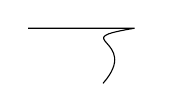
\begin{tikzpicture}[x=1cm,y=1cm]\draw (0,0)--(1.35,0) .. controls (.45,-.15) and (1.45,-.13) .. (.95,-.7);\end{tikzpicture}}

\uline{Corollaire} $\underline{\mathrm{Hom}}_{\deleted{\unsure{K}}L/K}(\deleted{\unsure{S}}\mathrm{Spec}_{\unsure{?|g}}(\deleted{\unsure{K}}L),X_{(L)})$ n'existe pas. À fortiori $\underline{\mathrm{Hom}}_K(\unsure{\mathrm{Spec}|\mathrm{Spm}}(L),X_{(L)})$ n'existe pas

On fera attention que dans cet exemple, $K$

% archive sheet number: 35
